\section{Project: Analyse blade grinder vibration}

\textbf{21022:} Here I'd like to talk a little about the difficulties encountered in the vibration analysis, such as my lack of knowledge of the subject, doubts about the reference system (local vs global),
the lack of real operational data and counter-intuitive results, and the need to strengthen the methodology and repeat the experiment

% \todo{Improve existing Industrial production}

\subsection{Initial Hypothesis}
\paragraph{Client} Stumabo International, a manufacturer of precision blades for the food processing industry, produces several million blades per year, 
and it is known in the industry for their progressive industrial potato cutting solutions, and innovative shapes produced through hydro-cutting systems.
Stumabo also uses their knowledge to integrate the best blade in the FAM industrial mechanical cutters~\cite{Misc:stumabo_en_website}.

\paragraph{Context/Intro: Machine line}
\begin{figure}[ht]
    \begin{subfigure}{\textwidth}
        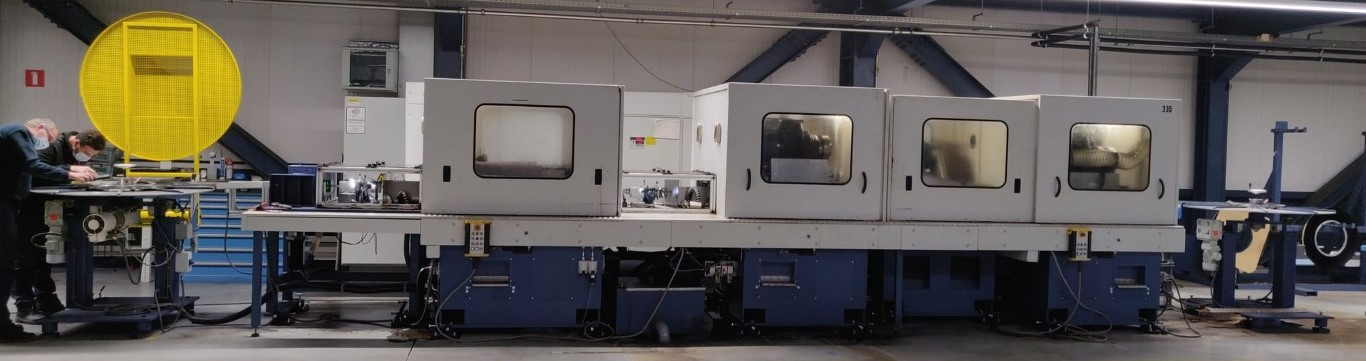
\includegraphics[width=\linewidth]{stumabo/installation/line_photo.jpg}
        \caption{Line overview: side view}
        \label{fig:line_overview}
    \end{subfigure}
    \begin{subfigure}{\textwidth}
        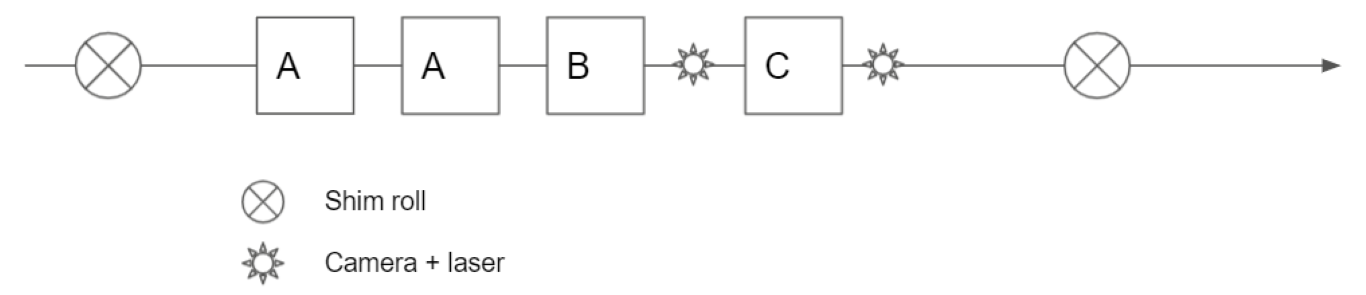
\includegraphics[width=\linewidth]{stumabo/installation/line_schematics.png}
        \caption{Line motor schematics}
        \label{fig:line_schematics}
    \end{subfigure}
    \caption{Stumabo's blade production line covered by this project}
    \label{fig:stumabo_prod_line}
\end{figure}

As shown in figure~\ref{fig:stumabo_prod_line} there are four different stations (\subref{fig:line_overview}) with each one or two motors type ${A,B,C}$ (\subref{fig:line_schematics}).
Each station has grinding stones to sharpen a blade, which is one long strip of steel passing through all the machines.
To perform their grinding task, the stones turn around their axe sharpening the steel blade, each machine in its own way.

\subsection{Goal(s), purpose \& critical factors}
The project started in conjunction with the beginning of my internship experience (Oct-Nov 2021), and I had the pleasure of contributing in its early stages (\textit{ad-hoc} campaign);
\todo{DG: dare definizione di campagna ad hoc?}
unfortunately my practice ended before the second, more substantial phase of the project began (April 2022).
Let's see what the goals are in the long and short term and then exploring the latter.
\paragraph{Long Term: Project lifecycle}
\begin{itemize}
    \item[$\circledcirc$] Increase production quality through the use of continuous data analysis.
    \item[$\circledcirc$] Avoid unplanned standstill (downtime) by preventing critical components failure.
    \item[$\circledcirc$] Extends the life of machines and installation through \acl{PdM} and \acl{cm} (see Section \ref{section:maintenance})
\end{itemize}
\paragraph{Short Term: \textit{ad-hoc} campaign}
\begin{itemize}
    \item[$\circledcirc$] It is possible to identify a strong impact of the turning of the grindstones? Perhaps a possible imbalance?
    \item[$\circledcirc$] As a general insight, do we have indication that something is causing strong vibration?
    \item[$\circledcirc$] Lastly, as preliminary path for the \ac{CtM}, identify purpose.
\end{itemize}

\subsection{Project description by phases}
\begin{figure}[ht]
    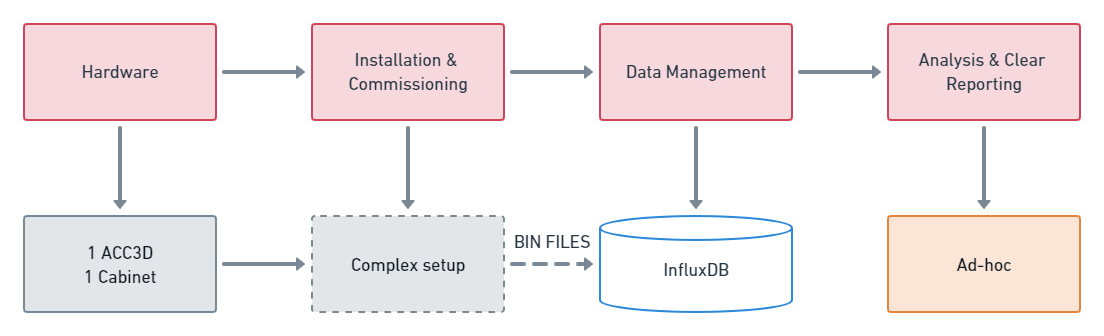
\includegraphics[width=\textwidth]{stumabo/21022_STU.png}
    \caption{Core Stages of this (full) project}
    \label{fig:stumabo_stages}
\end{figure}
As we saw together in section~\ref{section:zensor_approach}, we can have approximately two types of projects and this one a complete one.
However, as the reader will have already guessed, being a preparation campaign, as mentioned earlier, it will have less complexity than a big project.
My contribution was to help with the analysis phase, but it's important to emphasize how the first three phases went, because they will have serious implications for data development and analysis.

% \begin{wrapfigure}{l}{.25\textwidth}
%     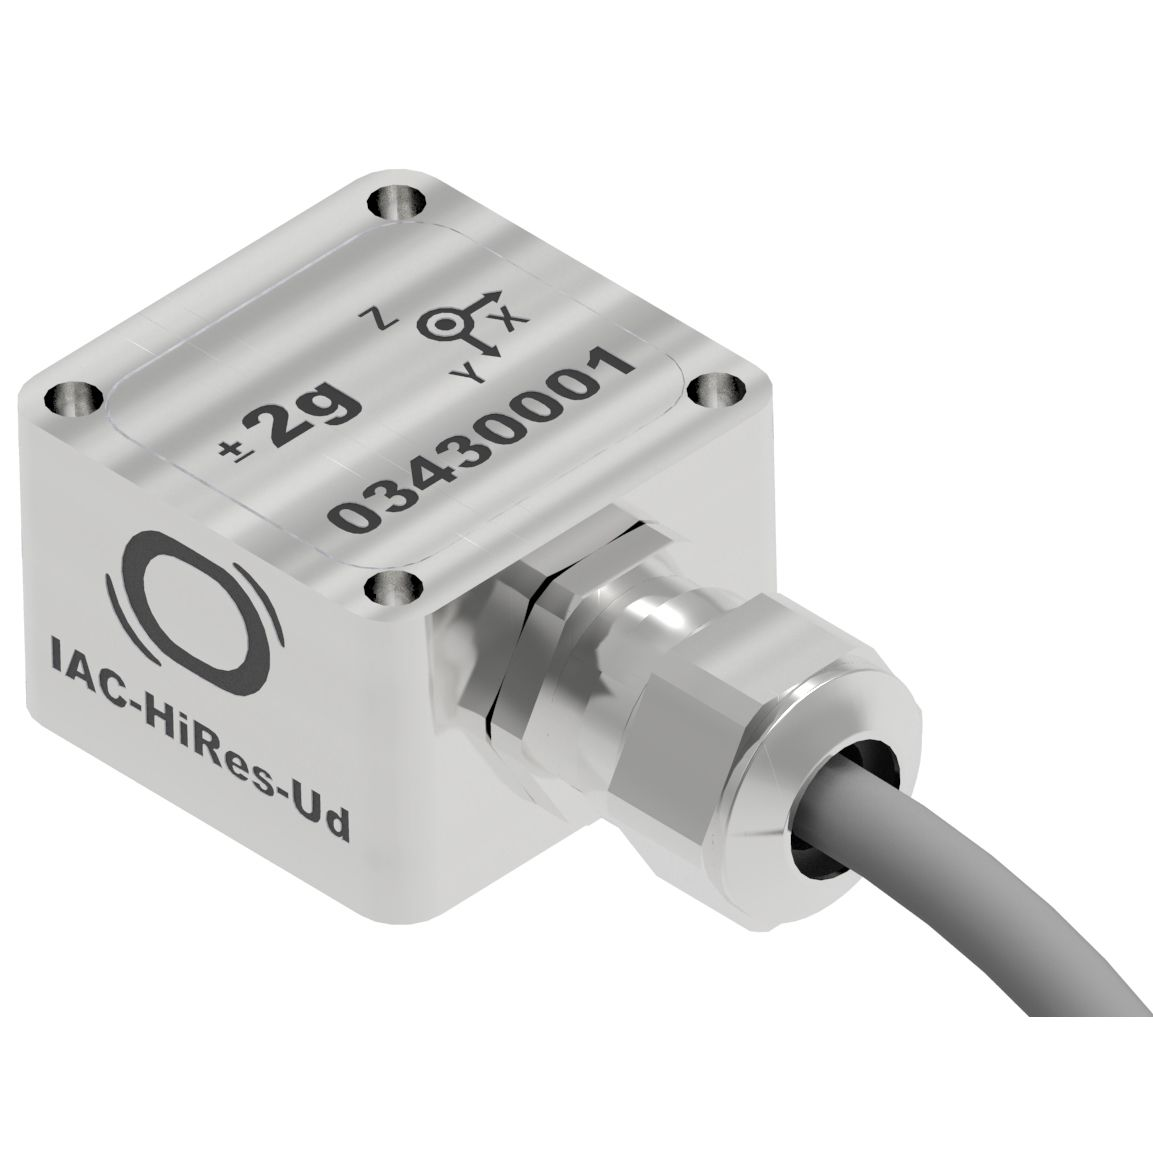
\includegraphics[width=.25\textwidth,height=.25\textwidth]{stumabo/installation/accelerometer_3_axis.jpg}
%     \caption{An industrial ACC3D}
%     \label{fig:stumabo_acc3d}
% \end{wrapfigure}

\paragraph{Hardware} One 3-dimension accelerometer, called \textit{ACC3D} in Figure \ref{fig:stumabo_acc3d}, and a ``mobile cabinet'' was provided to Stumabo, 
which they placed on each of the four machine and roughly kept track of the different positions and operations in a log file.
Unfortunately this is the only operational data available, with the following structure (see Table \ref{tab:stu_logfile}).
As you can see, despite being in Flemish, it has several tags but with one big issue: start and end time are approximate and do not reflect the data trends collected by the above-mentioned sensor.
More on that later on. 

\begin{table}[h]
    \centering
    \begin{tabularx}{\textwidth}{llllll}
        \toprule
        Datum & Start tijd & Stop tijd & Actie & Opmerkingen & Opstelling \\\midrule
        \textit{Date} & \textit{Start time} & \textit{Stop time} & \textit{Action} & \textit{Notes} & \textit{Setup} \\\midrule
        08/10/2021 & 13:19 & 13:29 & Test & Enkel \dots & grote \dots \\ % de slijpstenen van station 1 (grote snede blauwe zijde) draaien. & grote snede blauw  \\ 
        \midrule
        \dots & \dots & \dots & \dots & \dots & \dots \\\midrule
        30/11/2021 & 12:35 & 14:07 & Prod & \dots & \dots \\\bottomrule
    \end{tabularx}
    \caption{Log file structure}
    \label{tab:stu_logfile}
\end{table}

\begin{figure}[ht]
    \begin{subfigure}{0.33\textwidth}
        \centering
        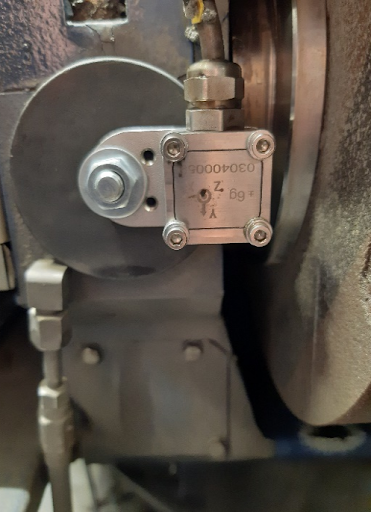
\includegraphics[height=\linewidth]{stumabo/installation/acc_station_1_blue.png}
        \caption{Installation photo}
        \label{fig:s1b_foto}
    \end{subfigure}
    \begin{subfigure}{0.33\textwidth}
        \centering
        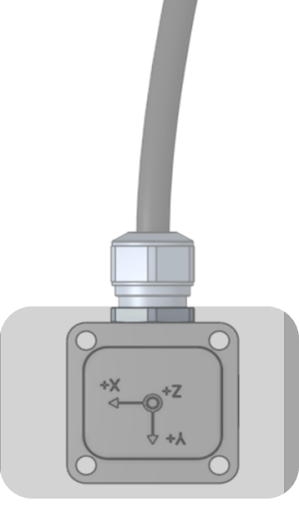
\includegraphics[height=\linewidth]{stumabo/installation/acc_render.png}
        \caption{CAD render}
        \label{fig:s1b_render}
    \end{subfigure}
    \begin{subfigure}{0.32\textwidth}
        \centering
        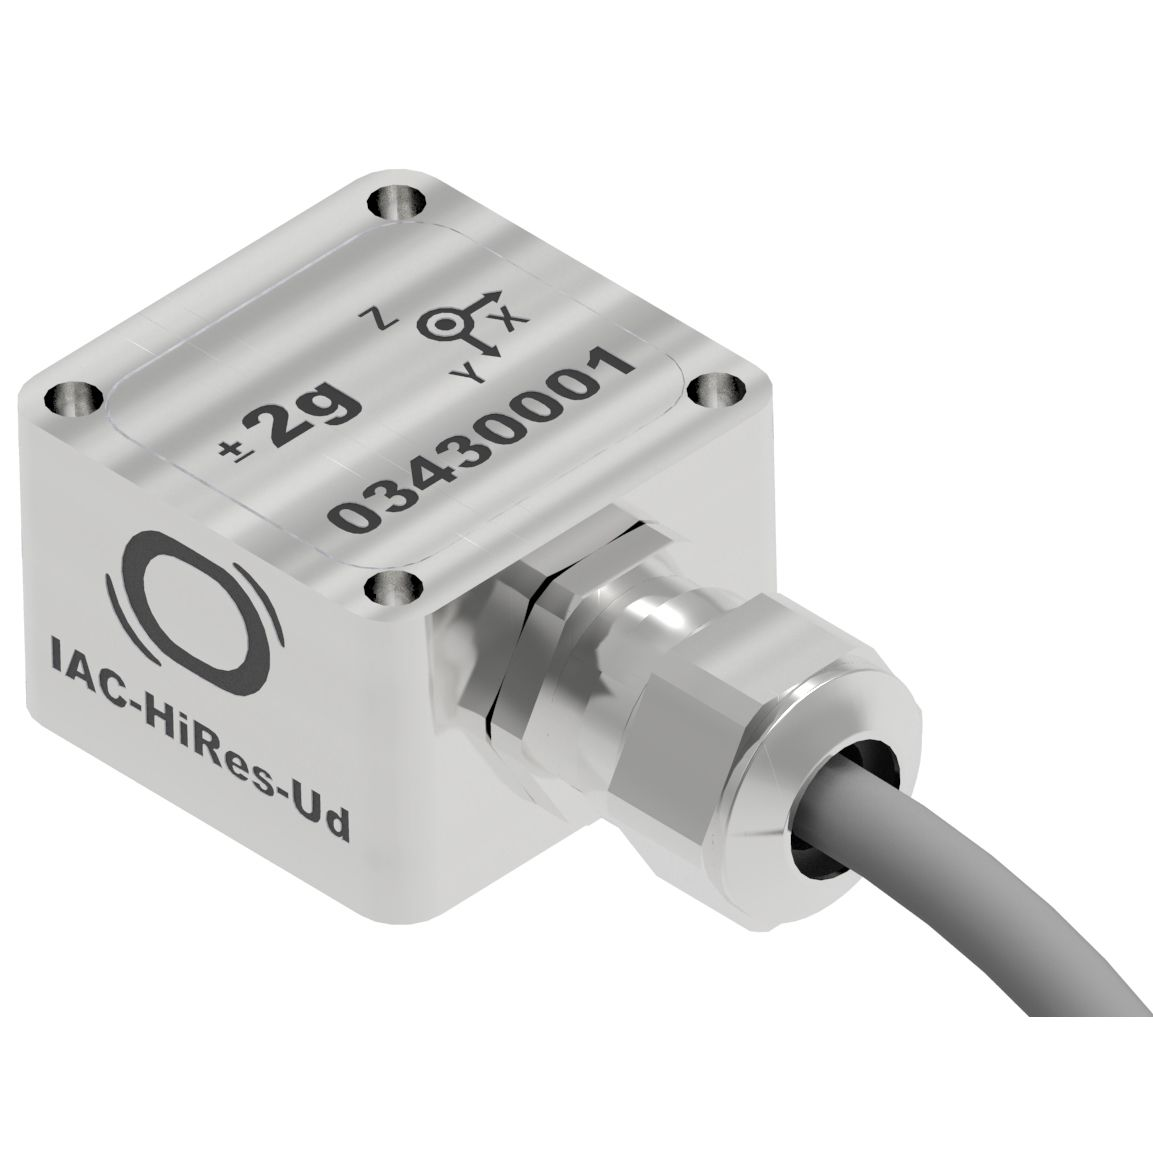
\includegraphics[height=\linewidth]{stumabo/installation/accelerometer_3_axis.jpg}
        \caption{An industrial ACC3D}
        \label{fig:stumabo_acc3d}
    \end{subfigure}
    \caption{Station 1 \textcolor{blue}{blue} side setup}
    \label{fig:stu_station1_b}
\end{figure}

\paragraph{Installation} We must therefore clarify, before we go any further, the industrial setup: in our aid, come the engineering schematics showed in figure \ref{fig:engineering_files};
it consists in three subfigures: the first one (\subref{fig:top_view_line}) represents the same production line we saw earlier at \ref{fig:line_overview}, just from another prospective. 
This view from above makes it easier for us to identify some important elements. 
It is essential to clarify a convention a simple convention: within Stumabo the right side of the line is referred to as \textcolor{red}{red}, \textit{rood} in Flemish, and, in the same way, 
the left side will be referred to as \textcolor{blue}{blue}, \textit{blauw}. 
We can now make a direct connection with Figure (\subref{fig:blade_evolution}), which shows us the evolution of the blade during the process.
First it is sharpened, from the 1st \textcolor{blue}{blue} station, on the left side, and then it passes to the 1st \textcolor{red}{red} station, where it will be rolled on the right side. 
Same goes for 2nd and 3rd station, that have two grinders aligned.
Finally, we have Schema (\subref{fig:local_to_global}) which represents in more detail how the sensor has been installed and what consequences it has with respect to the coordinate system, 
a somewhat complex issue that has caused several headaches in the analysis phase. This would therefore appear to be a good point to take stock of the situation.

\begin{figure}[ht]
    \begin{subfigure}{\textwidth}
        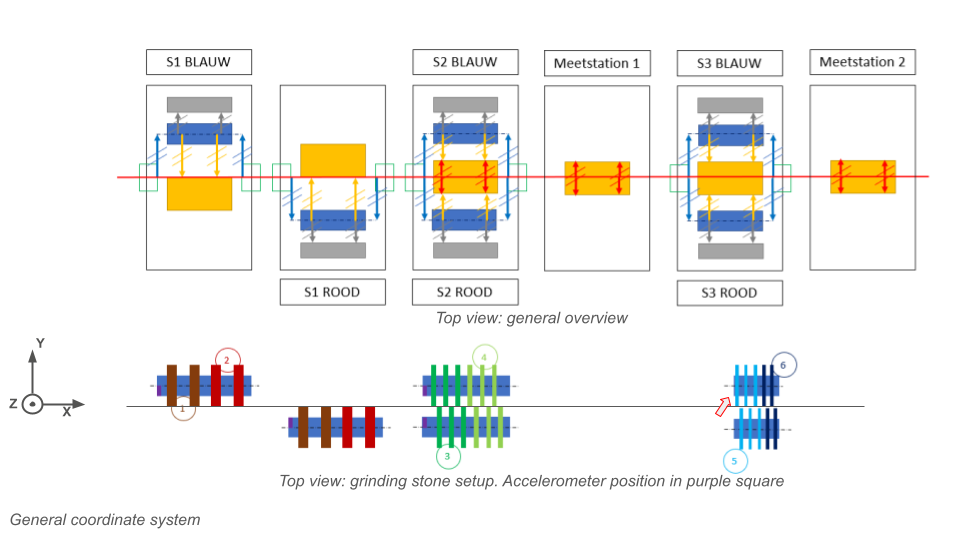
\includegraphics[width=.9\linewidth]{stumabo/installation/general_cordinate_system.png}
        \caption{Top view overview of stations plus grinding stones detail.
            Purple dots on the bottom details are where the $3D$ accelerometer was placed}
        \label{fig:top_view_line}
    \end{subfigure}
    \begin{subfigure}{\textwidth}
        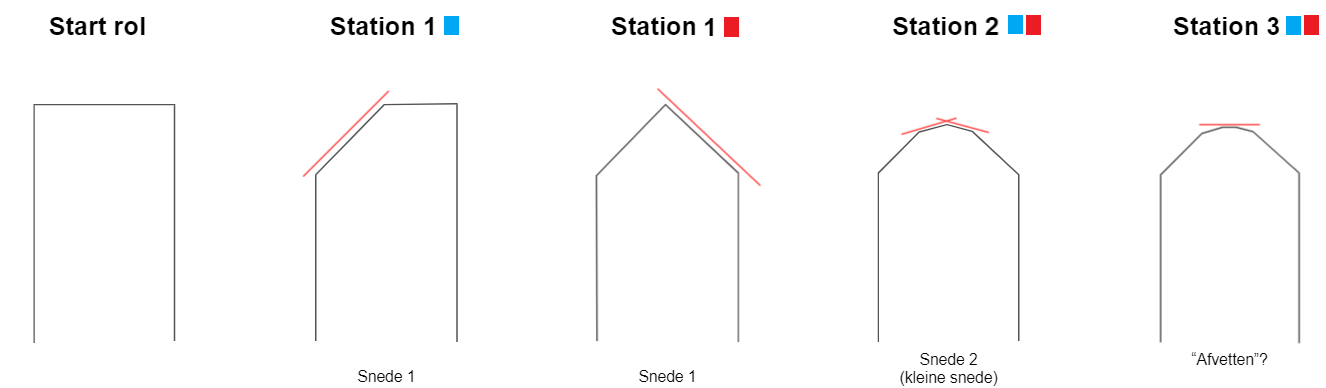
\includegraphics[width=.9\linewidth]{stumabo/installation/blade_processing.png}
        \caption{Blade evolution, a sketched overview of the cut by station}
        \label{fig:blade_evolution}
    \end{subfigure}
    \begin{subfigure}{\textwidth}
        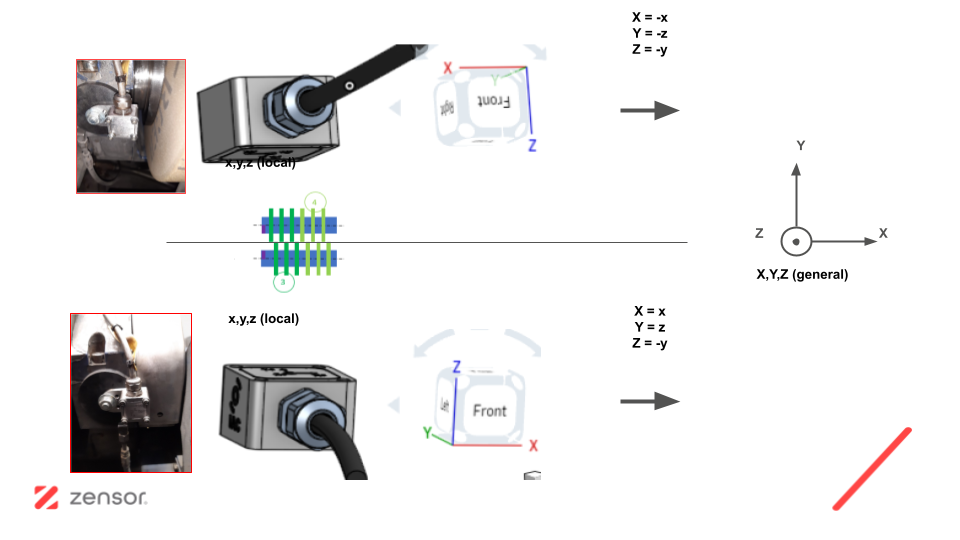
\includegraphics[width=.9\linewidth]{stumabo/installation/local_to_global.png}
        \caption{From local to general coordinate system, top view}
        \label{fig:local_to_global}
    \end{subfigure}
    \caption{Engineering schematic are also important during analysis}
    \label{fig:engineering_files}
\end{figure}

The accelero was installed within the line, adjacent to the stones and close to the blade, by means of a round magnet, as shown in Figure \ref{fig:s1b_foto}.
This was installed, at different times in different stations mirrored on both sides, except the last one, for a total of five different locations 
${S_{1}\textcolor{red}{R}\&\textcolor{blue}{B}, S_{2}\textcolor{red}{R}\&\textcolor{blue}{B}, S_{3}\textcolor{blue}{B}}$ as shown in the bottom part of Figure \ref{fig:top_view_line}.
It follows that two different reference systems are present:
\begin{itemize}
    \item local $(x,y,z)$ for each sensor placement;
    \item global $(X,Y,Z)$ for the entire production line.
\end{itemize}
The most attentive reader will have already grasped the different references present in the previously mentioned figures.
This dual model well abstracts the reality, but does not allow to compare the various stations, ergo to achieve one of the initial goals.
So it will be necessary to report everything in global coordinates, taking into account two added factors: sensor orientation and installation angle. 

\begin{itemize}
    \item \textbf{Sensor Orientation} 
    Keeping our attention on Figure \ref{fig:stu_station1_b}, we can see how the sensor has been installed horizontally, with the $x$-axis as parallel as possible to the blade ($X$) with 
    the help of a level. This tolerating some errors due to disturbing factors such as color, dirt and imperfections of the metal.
    Furthermore, the latter is installed upside down, i.e.\ parallel to the $Z$ axis as shown \ref{fig:s1b_render}.
    \item \textbf{Installation Angle}
    You also have to take into account that the machines have various angles to the ideal $Z$-axis, this was measured on site and varies from station to station, from 5° to 12° degrees.
\end{itemize}
We will delve into both aspects in the final stage of analysis, but now the following equation-mapping (\ref{eq:op}) from local to global coordinate should be clear, 
where $\widehat{widehat}$ stands for the \textit{rotation} operator and $\underline{underline}$ for \textit{transposition}.
\begin{equation}
    \left\{ \begin{array}{cl}
        x = \alpha & \Rightarrow  \ x = \widehat{\alpha} \ \Rightarrow  \ X = \underline{\widehat{\alpha}} \\
        y = \beta & \Rightarrow  \ y = \widehat{\beta} \ \Rightarrow  \ Y = \underline{\widehat{\beta}} \\ 
        z = \gamma & \Rightarrow  \ z = \widehat{\gamma} \ \Rightarrow  \ Z = \underline{\widehat{\gamma}}
        \end{array} \right.
    \label{eq:op}
\end{equation}
Hoping that this idea is clear to the reader we move on to the following phase.

\paragraph{Data Management}
As stated previously a single sensor was placed in different locations, remaining on for the duration of the ad hoc project. We will therefore have a single data stream.
The data flow is as follows: from the sensor to the cabinet to AWS and, finally, InfluxDB.
I would like to point out that, at cabinet level, two separate binary files are created, where $x$ and $z$ channels are aggregated together and, instead $y$ channel is kept separated. 
Moreover, for each sensor channel, all vibrations are recorded at $60hz$, or 60 points per second, for a total of 180 per second.
As you can easily imagine when you want to visualize, e.g.\ doing some \ac{EDA} as discussed in subsection \ref{subsubsec:eda}, 
and investigate hours and hours of data these are way too many data points.
This is the reason why Lambda, during data ingestion, aggregates the data using the mean function, and reduces the frequency to $1hz$, i.e.\ 
performs a down sampling operation. It then saves both streams in the \ac{tsdb} as separate measurements. This is an important detail that will be useful later.

%\subsection{Resources needed (to accomplish my task)}

% Before starting the actual monitoring campaign there has been an “ad-hoc” measurement campaign. One accelerometer + “mobile cabinet” *(the previous SST cabinet + ACC)* was provided to Stumabo, 
% which they placed on each machine and kept track of the different positions and operations in a log (Excel). RMS values were extracted by Damiano Gianotti and insights were derived by Yves (January 2022).

% A potential deeper investigation for the ad-hoc data is being proposed as of February 2022

% \begin{figure}[ht]
%     \begin{subfigure}{0.5\textwidth}
%         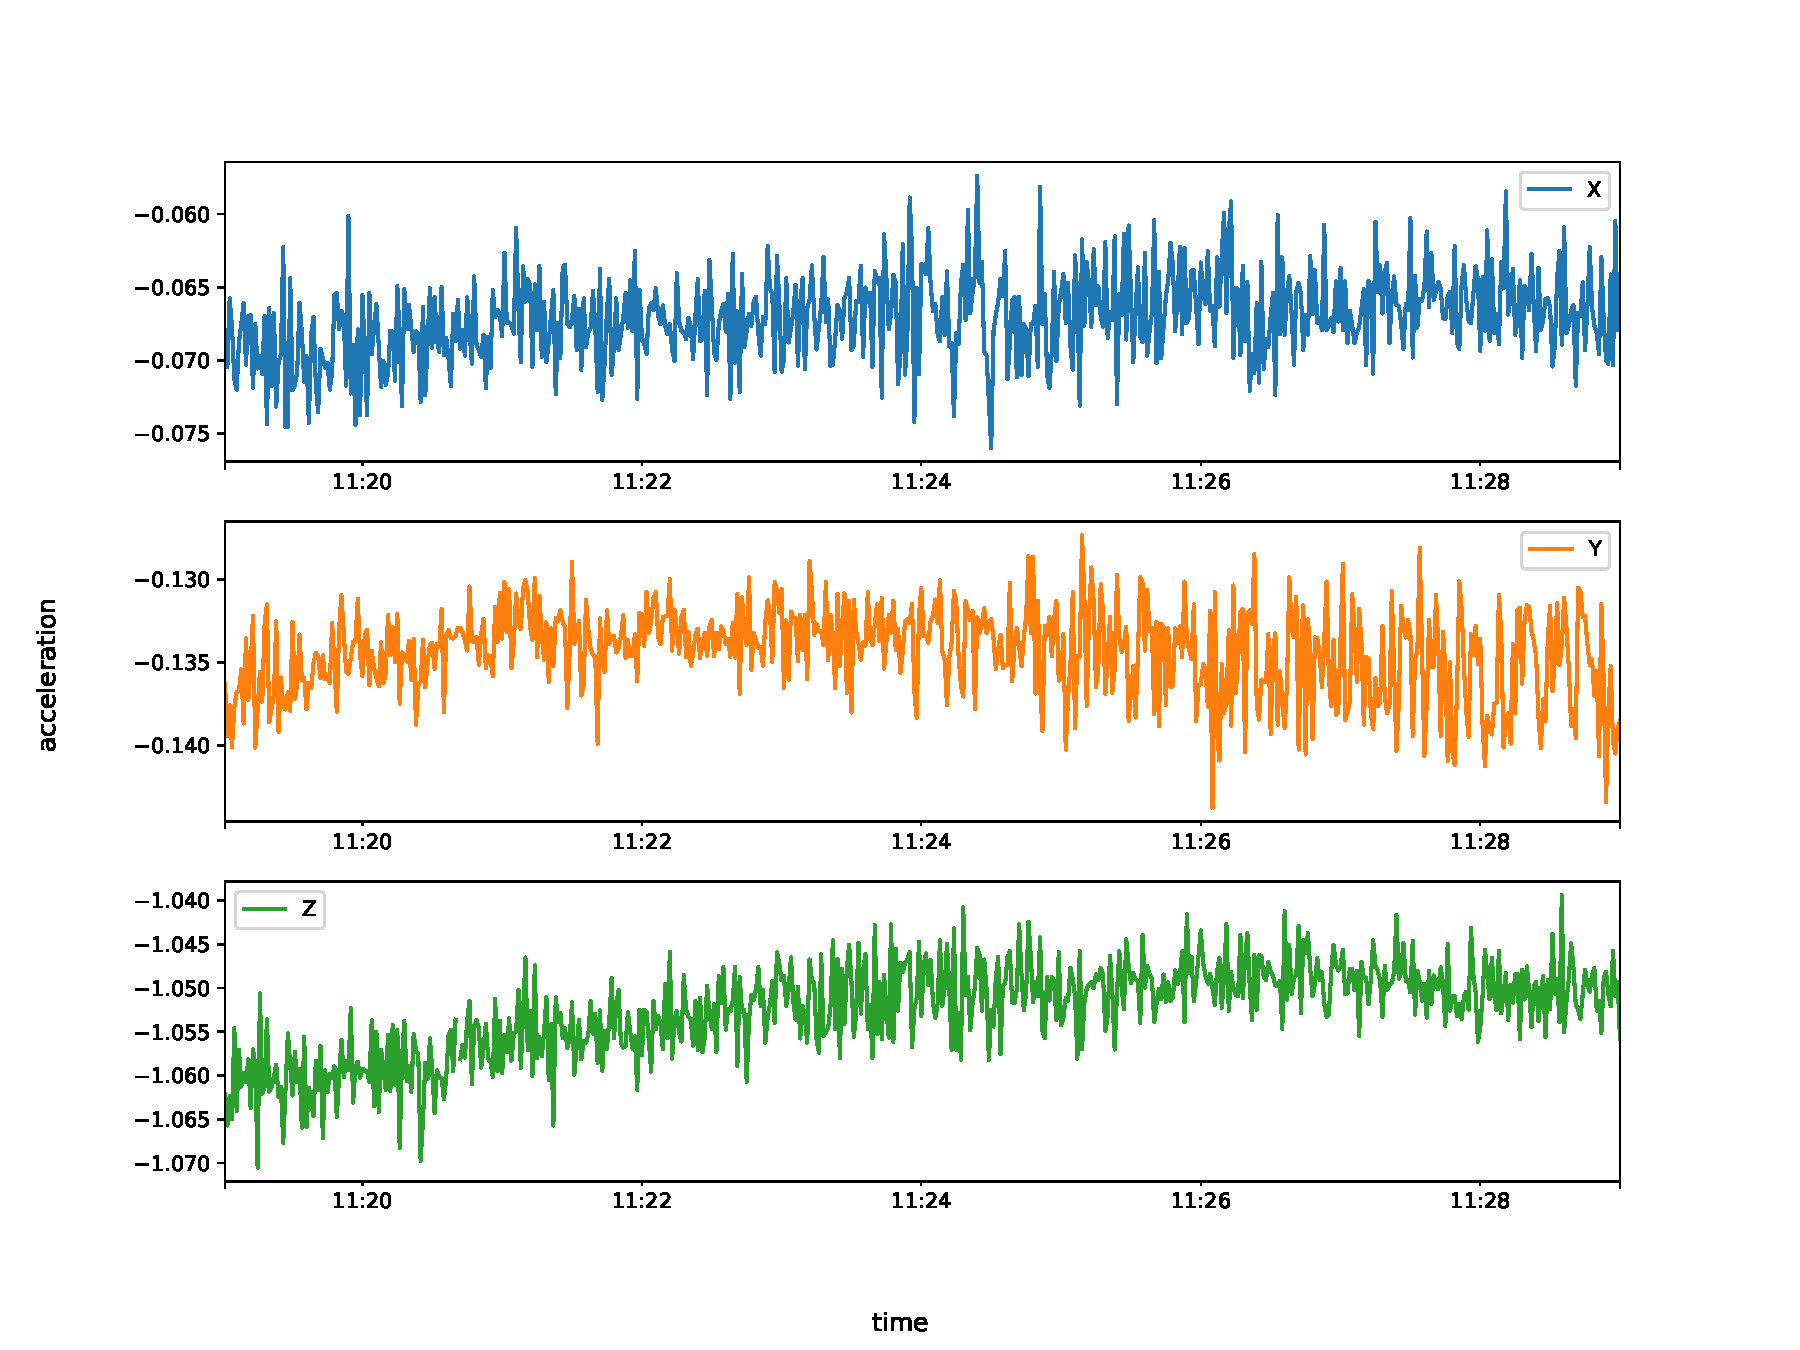
\includegraphics[width=\linewidth, height=6cm]{1hz-raw-vibration.pdf} 
%         \caption{Caption1}
%         \label{fig:subim1}
%     \end{subfigure}
%     \begin{subfigure}{0.5\textwidth}
%         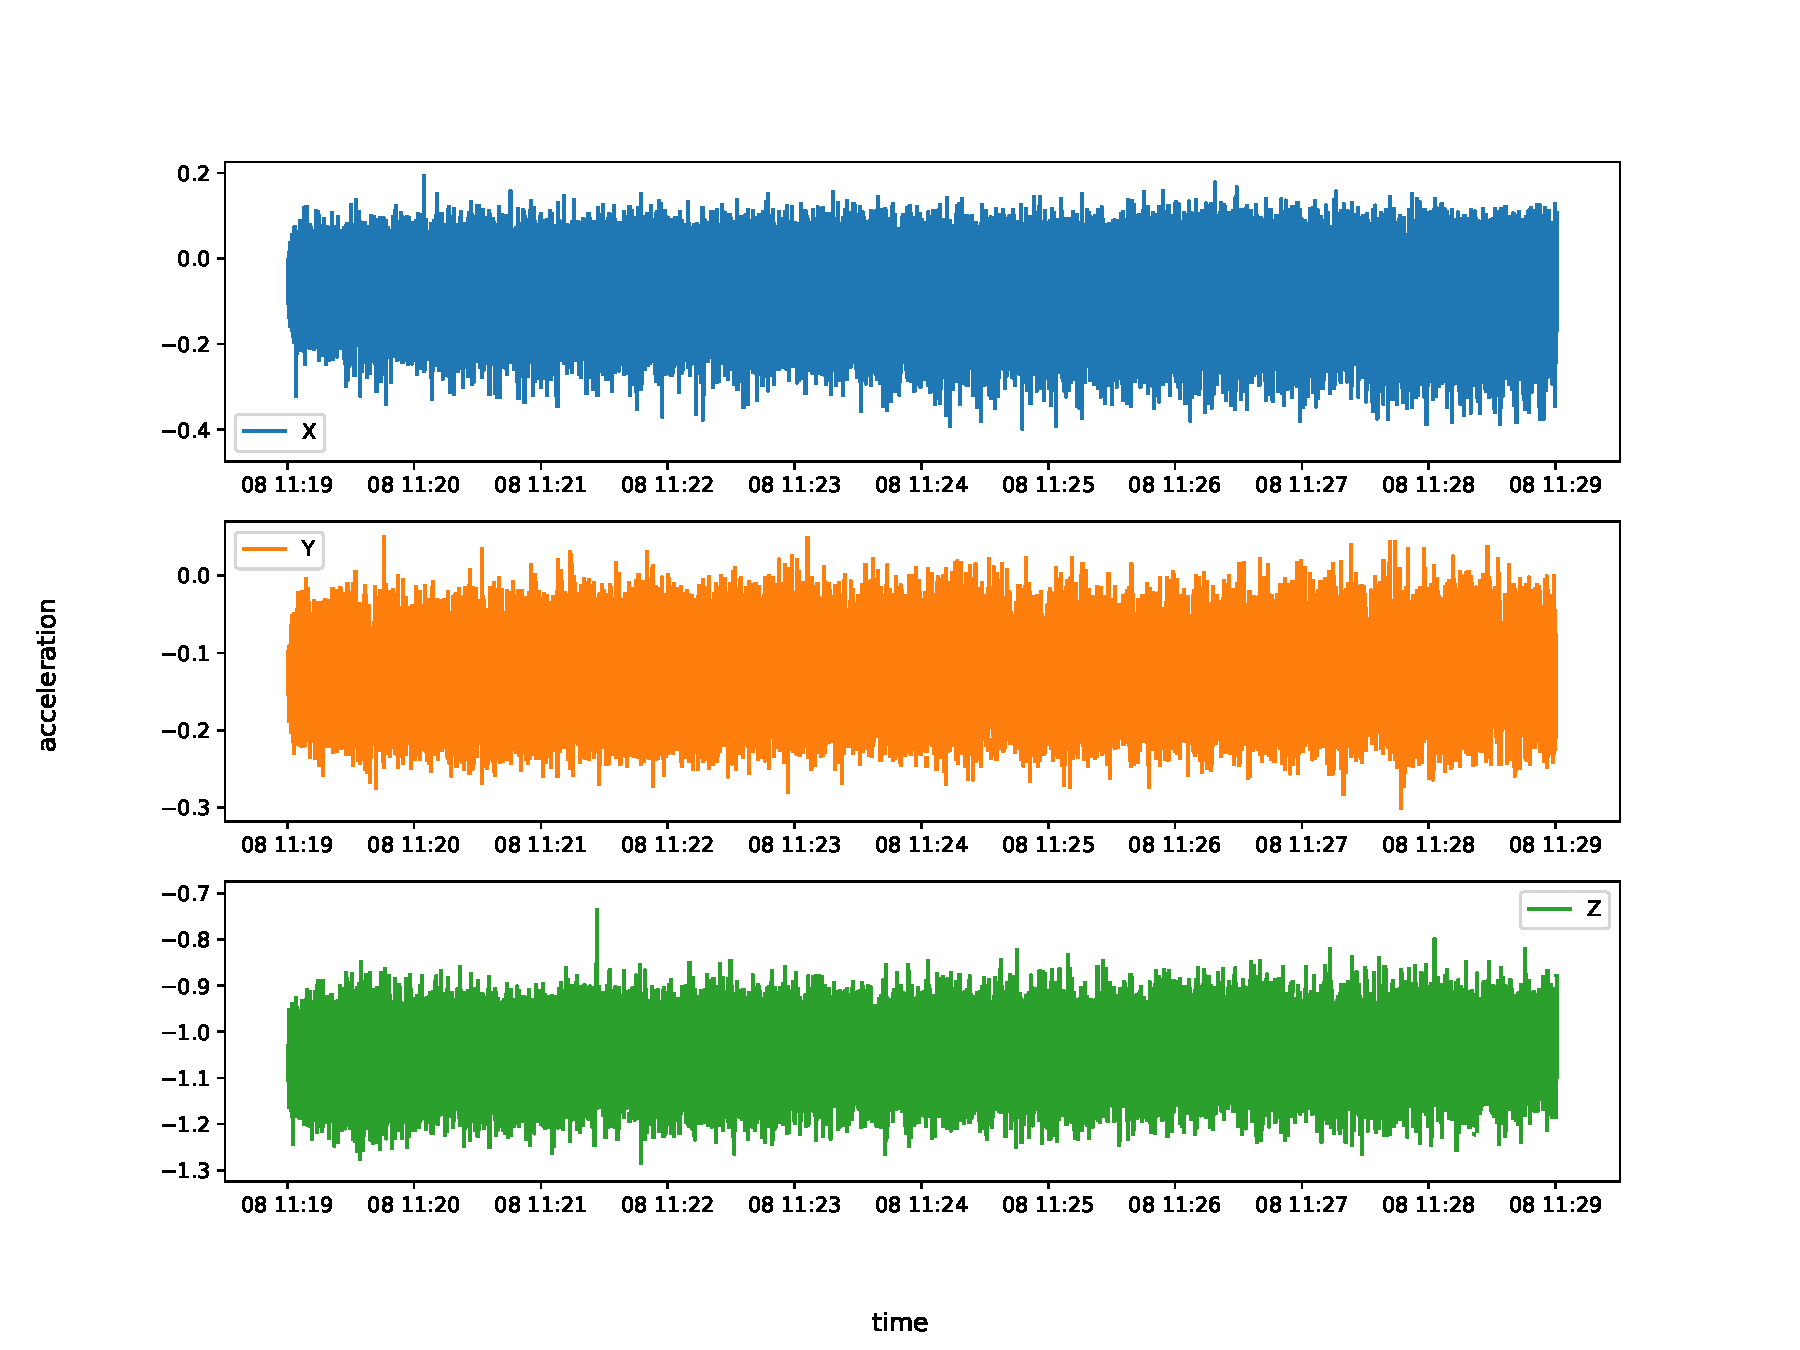
\includegraphics[width=\linewidth, height=6cm]{60hz-raw-vibration.pdf} 
%         \caption{Caption2}
%         \label{fig:subim2}
%     \end{subfigure}

%     \caption{Caption for this figure with two images}
%     \label{fig:image2}
% \end{figure}

% \begin{table}[h]
%     \centering
%     \begin{tabularx}{\textwidth}{@{}lllllllll@{}}
%     \toprule
%     start & einde & actie & kant & stat & draaien & $X$ & $Y$ & $Z$ \\ \midrule
%     13:19:01 & 13:29:01 & TEST & \textcolor{blue}{B} & 1 & 1 & 131 & 176 & 592 \\ 
%     13:29:01 & 13:39:00 & TEST & \textcolor{blue}{B} & 1 & 1,2 & 160 & 143 & 461 \\  
%     13:38:58 & 13:49:01 & TEST & \textcolor{blue}{B} & 1 & 1,2,3B & 132 & 166 & 356 \\ 
%     13:48:59 & 13:59:00 & TEST & \textcolor{blue}{B} & 1 & 1,2,3R & 113 & 149 & 244  \\
%     13:59:00 & 14:08:59 & TEST & \textcolor{blue}{B} & 1 & 1,2,3B,3R & 145 & 143 & 217 \\ 
%     14:09:00 & 14:20:00 & TEST & \textcolor{blue}{B} & 1 & 1,2,3B,3R,4 & 176 & 153 & 294 \\ 
%     \dots \\
%     10:04:00 & 12:35:00 & DASTE & \textcolor{blue}{B} & 3 & 1,2,3B,3R,4 & 630 & 542 & 1489 \\
%     \bottomrule
%     \end{tabularx}
%     \caption{I valori vanno presi con $10^{-6}$}
%     \label{tab:my-table}
% \end{table}